\subsection{GameLoop}\label{sec:runtime_gameloop}

Die \texttt{GameLoop} in \textit{helios} integriert die verschiedenen Systeme, die das Verhalten der spielspezifischen \texttt{GameObject}s steuern.
Sie ist in die Phasen \texttt{Pre}, \texttt{Main} und \texttt{Post} unterteilt, was eine klare Verortung von Spiellogik, Physik-Simulation, Kollisionserkennung, Synchronisation des \texttt{SceneGraph} sowie weiterer für die Spielmechanik relevanter Systeme erlaubt.
Die Unterteilung in diese drei Phasen ist dabei eher konzeptionell und ermöglicht eine semantische Gruppierung der Systeme nach ihrer Grundfunktionalität: State-Verarbeitung, Physik und Kollisionssystem, Aktualisierung von Spielmechaniken, Rendering sowie nachgelagertes Säubern von \textit{Dirty States}, damit Frame $N+1$ einzelne Komponenten nach einer erfolgten Bearbeitung wieder berücksichtigen kann.

\vspace{5mm}
\begin{tcolorbox}[title={Frame-Semantik}]
    Frame $N$ ist ein Schnappschuss der Welt zum Zeitpunkt $t$.
    Frame $N+1$ ist der Schnappschuss zum Zeitpunkt $t + \Delta t$.
    Dazwischen existiert für die Engine kein Zustand - die Welt wird ausschließlich in diskreten Schritten fortgeschrieben (\textit{Euler-Integration}).
\end{tcolorbox}
\vspace{5mm}


Die Phasen selbst sind in beliebig viele \textit{Passes} untergliedert.
Jeder Pass kann einem bestimmten Spielzustand zugeordnet werden, sodass keine unnötige Rechenzeit oder unbeabsichtigte Aktualisierungen stattfinden, wenn sich das Spiel bspw.\ im Pausenzustand befindet (siehe Abschnitt~\ref{sec:state_management}).
Ein Pass kann über einen \texttt{CommitPoint} von einem nachfolgenden Pass abgekoppelt werden, was es der Engine ermöglicht, den Inhalt der Nachrichtenpuffer zu tauschen und Nachrichten den nachgelagerten Passes zur Verfügung zu stellen: Hierbei tauschen die als \textit{DoubleBuffer} realisierten Puffer bei jedem \texttt{CommitPoint} ihren Inhalt (Kopie Write $\rightarrow$ Read, Leeren von Write), und alle Systeme können dabei ungestört aus einem Nachrichteneingang lesen, und in einen gesonderten Nachrichtenausgang schreiben.~\cite[S. 110]{Nys14}
Auf diese Weise bleibt der gewünschte Determinismus erhalten, wonach nach einem \texttt{CommitPoint} ein wohldefinierter Nachrichtenstand an die Systeme im darauffolgenden \textit{Pass} übergeben wird.

Dies führt das Konzept der Daten-Snapshots fort, die bereits an anderer Stelle in \textit{helios} klar voneinander abgegrenzte Verarbeitungsschritte erlauben, wie etwa der \texttt{SceneGraph}-Snapshot, der \texttt{Gamepad}-Snapshot oder Snapshots von Objekt-Pools.

Das Konzept der \texttt{GameLoop} ist in Abbildung~\ref{fig:gameloop} skizziert.

\begin{figure}[htbp]
    \centering
    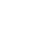
\includegraphics[width=0.8\textwidth]{content/de/architektur/runtime/img/gameloop.png}
    \caption{Skizze der \texttt{GameLoop} in \textit{helios}, die die Unterteilung in Phasen und Passes sowie die Zuordnung von Systemen zu den verschiedenen Passes darstellt. (Quelle: Eigene Darstellung)}
    \label{fig:gameloop}
\end{figure}

Ein wesentlicher Bestandteil der \texttt{GameLoop} ist der \texttt{UpdateContext}, der bei jedem Aufruf der in einem Pass registrierten Systeme übergeben wird und folgende Informationen beinhaltet:

\begin{itemize}
    \itemsep0.5em
    \item \texttt{ResourceRegistry}: Referenz auf die von der \texttt{GameWorld} verwalteten Ressourcen, um über den Engine-\texttt{CommandBuffer} Commands hinzufügen zu können.
    \item \texttt{EntityResolver}: Erlaubt die Validierung und Abfrage von \texttt{GameObject}s basierend auf \texttt{EntityHandle}s.
    \item \texttt{Session}: Eine Referenz auf das Session-\texttt{GameObject}, um Informationen über den derzeitigen State zu erhalten.
    \item \texttt{DeltaTime}: Die vergangene Zeit seit dem letzten Frame.
    \item \texttt{TotalTime}: Die vergangene Zeit seit Spielbeginn.
    \item \texttt{PhaseEventBus}, \texttt{PassEventBus}, \texttt{FrameEventBus}: Lese- und Schreib-Senken (\texttt{ReadSink}/\texttt{WriteSink} im Code, also Views für den Lese- bzw.\ Schreibpuffer), eingeteilt nach Phase, Pass und Frame, um gezielt Nachrichten weiterzuleiten.
    \item \texttt{InputSnapshot}: Der \texttt{InputSnapshot}, der Informationen über den Zustand des Eingabegeräts (hier: über \texttt{glfw} ausgewertetes Gamepad) beinhaltet.
    Die Snapshots beinhalten bereits die Information, ob Eingaben \textit{edge-triggered}, seit längerer Zeit oder gerade erst aktiviert worden sind.
    \item \texttt{ViewportSnapshots}: Zustand der im aktuellen Frame angezeigten Viewports als Szenenrepräsentanten.
    Diese werden u.\,a.\ von dem \texttt{UiTransformSystem} benötigt, um eine Zuordnung von UI-Komponenten zu derzeitig angezeigten Viewports zu ermöglichen.
    \item \texttt{Level}: Ein Zeiger auf das \texttt{Level}, in dem u.\,a.\ die Bounds festgehalten sind; relevant für Kollisions- und Bewegungssysteme.
\end{itemize}

\vspace{5mm}
\begin{tcolorbox}[title={Technical Debt der GamLoop}]
Die \texttt{GameLoop} berücksichtigt zur Aktualisierung der Spielmechaniken allein den von außen übergebenen $\Delta t$.
Damit fehlen eine idiomatische Synchronisation der Zeitschritte sowie eine Interpolation bei den Framewechseln.\\

Dies wird allgemein als Anti-Pattern verstanden, da es zu unvorhersehbarem Verhalten kommt: Die Simulation der Spielwelt wird hierdurch von der \textit{Framerate} abhängig~\cite{FixYourTimestep}~\cite[S. 136]{Nys14}.\\

In der zum Zeitpunkt der Veröffentlichung dieses Dokuments verfügbaren Version von \textit{helios} lässt sich der entsprechende Seiteneffekt in der \textit{Scoring Demo} nachvollziehen.
Läuft im Titelscreen die Animation der NPC-Objekte und wird das darstellende Fenster mit der Maus bewegt, wird der Main-Thread der Anwendung - und damit auch die interne Zeitmessung - angehalten.
Nach erneuter Aktivierung des Fensters muss dann ein unverhältnismäßig großer Zeitschritt verarbeitet werden, was sich durch Sprünge in den Animationen und Positionen der NPCs bemerkbar macht.\\

Damit wird letztendlich ein deterministisches Simulationsverhalten unterbunden, obwohl ein Teil der Implementierung (fixe Reihenfolge der Systeme der GameLoop, Definition der \textit{CommitPoints}) gerade dies zum Ziel hat.
\end{tcolorbox}
\vspace{5mm}





